%----------------------------------------------------------------------------
\chapter{Motivációs példa}
%----------------------------------------------------------------------------
A félévben végzett munkám reprezentálására egy EMF-ben készített, gólyatábor témájú modellt használtam.

%----------------------------------------------------------------------------
\section{Metamodell}
%----------------------------------------------------------------------------
A modell gyökérosztálya maga a tábor, ami tartalmazza a gólya és a senior osztályokat, valamint egymásba ágyazva a „szín” és a „szoba” osztályokat, ezekbe a csoportokba tartoznak a résztvevők. Minden csoport tartalmaz referenciát egy-egy megfelelő típusú seniorra, aki azt irányítja. A seniorok között kétirányú referencia található, a „színseniorok” és a „szobaseniorok” hierarchiájának ábrázolására.

\begin{figure}[H]
	\centering
	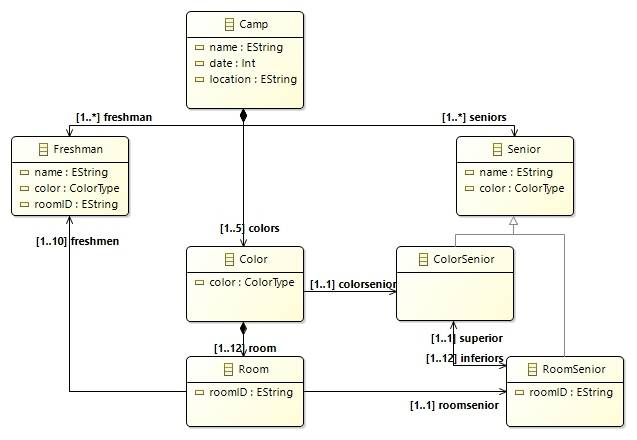
\includegraphics[width=150mm, keepaspectratio]{figures/metamodel.jpg}
	\caption{A gólyatábor metamodellje}
	\label{fig:metamodel}
\end{figure}


%----------------------------------------------------------------------------
\section{Példánymodell}
%----------------------------------------------------------------------------
Az előbbi metamodellnek egy lehetséges példánymodelljében egy kék és egy sárga szín van, mindegyik két-két szobával, valamint a megfelelő típusú senior vezetővel. Ezen a modellen egy hozzáférési szabály lehet a következő: mivel a Zsolti nevű kék színsenior a saját színén belül a szobaseniorok főnöke, ezért azt szerettem volna meghatározni, hogy ő - mint felhasználó - ezekhez az objektumokhoz férjen hozzá és módosíthassa őket.

\begin{figure}[H]
	\centering
	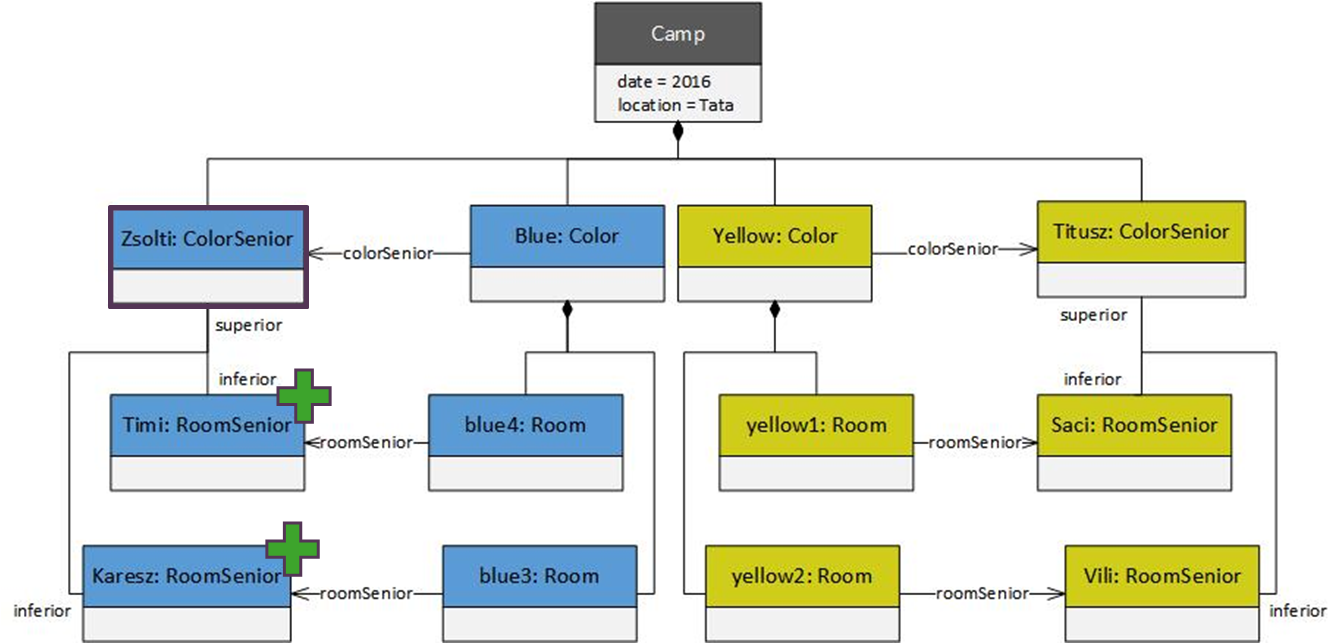
\includegraphics[width=150mm, keepaspectratio]{figures/instance.png}
	\caption{A gólyatábor példánymodellje az érvényesíteni kívánt szabállyal}
	\label{fig:instance}
\end{figure}
